\chapter[%
    Combinação da Primeira e Segunda Leis%
]{%
    Combinação da Primeira e da Segunda Leis
    da Termodinâmica%
}   \label{chap:exergyAnalysis}

    Ao contrário do que o aluno muitas vezes pensa, as duas Leis da
    Termodinâmica nasceram praticamente juntas e devem ser satisfeitas
    conjuntamente. A violação da primeira lei constitui um moto perpétuo de
    primeira espécie, ao passo que a violação da segunda lei constitui um moto
    perpétuo de segunda espécie.

    Considerando então que todos os processos entre dois estados de um sistema
    qualquer aberto ou fechado devem satisfazer simultaneamente a Primeira e a
    Segunda Lei, no que estamos realmente interessados agora é na capacidade ou
    potencial de realizar o trabalho que as transformações de estado encerram.

    Seja um reservatório térmico à temperatura \gls{temperature}. Se extrairmos
    o calor \gls{heatTransfer} do reservatório, a segunda lei nos proíbe de
    transformar, através de um processo cíclico, todo o \gls{heatTransfer} em
    trabalho \gls{workTransfer}, sem rejeitar pelo menos algum calor
    \gsub{heatTransfer}{environmentState} para o meio-ambiente. Pois bem, em
    relação ao reservatório do meio-ambiente a
    \gsub{temperature}{environmentState}, qual é o máximo trabalho que poderia
    potencialmente ser recuperado?

    Já aprendemos, quando estudamos o Ciclo de Carnot, que, para o reservatório
    a \gls{temperature} trocando reversivelmente o calor \gls{heatTransfer}, em
    relação ao meio-ambiente a \gsub{temperature}{environmentState} a máxima
    capacidade de realizar trabalho será dada por:
    %
    \begin{equation} \label{eq:4.1}
        \gsuper{workTransfer}{reversible}
        =
        \gls{heatTransferRate}
        \left(
            1
            -
            \frac{
                \gsub{temperature}{environmentState}
            }{
                \gls{temperature}
            }
        \right)\,.
    \end{equation}

    Lembremos também que, ao mínimo valor do calor rejeitado para o
    meio-ambiente, \gsupsub{heatTransfer}{reversible}{envronmentState},
    corresponde ao máximo trabalho \gsuper{workTransfer}{reversible}.

    Considere agora na \cref{fig:controlVolumeInteractionsExergyAnalysis} um
    volume de controle, com múltiplas entradas e saídas de massa, trocando
    calor com vários reservatórios térmicos e também com o meio-ambiente.

    \begin{figure}[!htb]
        \caption{%
            Esquema de volume de controle e as interações na sua fronteira.
        }

        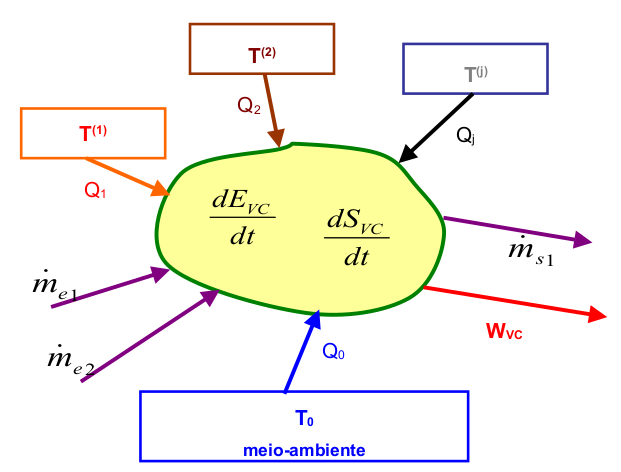
\includegraphics[
            width=\textwidth
        ]   {controlVolumeInteractionsExergyAnalysis.png}

        \label{fig:controlVolumeInteractionsExergyAnalysis}
    \end{figure}

    Vamos aplicar a Primeira Lei ao sistema aberto, isolando o trabalho
    mecânico:
	%
	\begin{equation} \label{eq:4.2}
        \gsub{workTransferRate}{controlVolume}
        =
        \underset{\gls{inlet}}{\sum }{
            \gsub{massFlowRate}{inlet}
            \left(
                \gls{intEnthalpy}
                +
                \frac{
                    \gls{velocityComp}^2
                }{
                    2
                }
                +
                \gls{gravityComp}
                \gls{zAxis}
            \right)_{\gls{inlet}}
        }
        -
        \underset{\gls{outlet}}{\sum }{
            \gsub{massFlowRate}{outlet}
            \left(
                \gls{intEnthalpy}
                +
                \frac{
                    \gls{velocityComp}^2
                }{
                    2
                }
                +
                \gls{gravityComp}
                \gls{zAxis}
            \right)_{\gls{outlet}}
        }
        +
        \underset{j \neq \gls{environmentState}}{\sum }{
            \gls{heatTransferRate}_{j}
        }
        +
        \gsub{heatTransferRate}{environmentState}
        -
        \DDt{\gsub{totalEnergy}{controlVolume}}\,.
    \end{equation}

    Agora, apliquemos a Segunda Lei ao mesmo sistema:
    %
    \begin{equation} \label{eq:4.3}
        \DDt{\gsub{entropy}{controlVolume}}
        =
        \underset{\gls{inlet}}{\sum }{
            \gsub{massFlowRate}{inlet}
            \gsub{intEntropy}{inlet}
        }
        -
        \underset{\gls{outlet}}{\sum }{
            \gsub{massFlowRate}{outlet}
            \gsub{intEntropy}{outlet}
        }
        +
        \underset{j \neq \gls{environmentState}}{\sum }{
            \frac{
                \gls{heatTransferRate}_{j}
            }{
                \state{\gls{temperature}}{j}
            }
        }
        +
        \frac{
            \gsub{heatTransferRate}{environmentState}
        }{
            \gsub{temperature}{environmentState}
        }
        +
        \gls{entropyCreatedRate}\,
        \,\,\,\,
        \text{com}
        \,\,\,\,
        \gls{entropyCreatedRate} \ge 0\,.
    \end{equation}

    Colocando, então, \gsub{heatTransferRate}{environmentState} em evidência em
    ambas as equações e igualando, obtemos:
    %
    \begin{equation} \label{eq:4.4}
    \begin{aligned}
        \underset{\gls{inlet}}{\sum }{
            \gsub{massFlowRate}{inlet}
            \left(
                \gls{intEnthalpy}
                +
                \frac{
                    \gls{velocityComp}^2
                }{
                    2
                }
                +
                \gls{gravityComp}
                \gls{zAxis}
                -
                \gsub{temperature}{environmentState}
                \gls{intEntropy}
            \right)_{\gls{inlet}}
        }
        &-
        \underset{\gls{outlet}}{\sum }{
            \gsub{massFlowRate}{outlet}
            \left(
                \gls{intEnthalpy}
                +
                \frac{
                    \gls{velocityComp}^2
                }{
                    2
                }
                +
                \gls{gravityComp}
                \gls{zAxis}
                -
                \gsub{temperature}{environmentState}
                \gls{intEntropy}
            \right)_{\gls{outlet}}
        }
        +\\
        &+\underset{j \neq \gls{environmentState}}{\sum }{
            \gls{heatTransferRate}_{j}
            \left(
                1
                -
                \frac{
                    \gsub{temperature}{environmentState}
                }{
                    \state{\gls{temperature}}{j}
                }
            \right)
        }
        -
        \DDt{}
        \left(
            \gls{totalEnergy}
            -
            \gsub{temperature}{environmentState}
            \gls{entropy}
        \right)_{\gls{controlVolume}}
        -
        \gsub{temperature}{environmentState}
        \gls{entropyCreatedRate}
        =
        \gsub{workTransferRate}{controlVolume}\,.\\
        \end{aligned}
    \end{equation}

    Vamos então supor como fixados: todas as propriedades das massas que entram
    e que saem; todos os fluxos de calor dos reservatórios a
    \state{\gls{temperature}}{j}; a variação das propriedades no interior do
    volume de controle. Em outras palavras, só podemos alterar
    \gsub{workTransferRate}{controlVolume}, \gls{entropyCreatedRate} e, em
    consequência da Primeira Lei, \gsub{heatTransferRate}{environmentState}.
    Podemos reestruturar a \cref{eq:4.2} como:
    %
    \begin{equation} \label{eq:4.5}
        \gsub{workTransferRate}{controlVolume}
        -
        \gsub{heatTransferRate}{environmentState}
        =
        C_1
    \end{equation}
    %
    onde $C_1$ é constante. Então, por causa da constante $C_1$, se tentarmos
    extrair mais potência \gsub{workTransferRate}{controlVolume} produzida pelo
    volume de controle, o fluxo de calor
    \gsub{heatTransferRate}{environmentState}, recebido do meio-ambiente a
    \gsub{temperature}{environmentState}, terá que aumentar conjuntamente. Como
    profissionais de energia, poderíamos perguntar-nos se poderíamos aumentar
    indefinidamente a potência produzida pelo sistema. A resposta limitante vem
    da Segunda Lei, pela expressão da \cref{eq:4.3}:
    %
    \begin{equation} \label{eq:4.6}
        \gsub{heatTransferRate}{environmentState}
        +
        \gsub{temperature}{environmentState}
        \gls{entropyCreatedRate}
        =
        C_2\,
        \,\,\,\,
        \text{com}
        \,\,\,\,
        \gls{entropyCreatedRate} \ge 0\,,
    \end{equation}
    %
    onde $C_2$ é uma outra constante. Concluímos então que, como
    \gsub{temperature}{environmentState} e \gls{entropyCreatedRate} são sempre
    positivos, o máximo \gsub{heatTransferRate}{environmentState} será obtido
    quando $\gls{entropyCreatedRate} = 0$, ou seja, quando todos os processos
    forem reversíveis. Nesse caso, $\gsub{heatTransferRate}{environmentState} =
    C_2$.

    A máxima potência, portanto,
    \gsupsub{workTransferRate}{reversible}{controlVolume} , será obtida
    fazendo-se $\gls{entropyCreatedRate} = 0$ na \cref{eq:4.4} e será dada por
    %
    \begin{equation} \label{eq:4.7}
    \begin{aligned}
        \underset{\gls{inlet}}{\sum }{
            \gsub{massFlowRate}{inlet}
            \left(
                \gls{intEnthalpy}
                +
                \frac{
                    \gls{velocityComp}^2
                }{
                    2
                }
                +
                \gls{gravityComp}
                \gls{zAxis}
                -
                \gsub{temperature}{environmentState}
                \gls{intEntropy}
            \right)_{\gls{inlet}}
        }
        &-
        \underset{\gls{outlet}}{\sum }{
            \gsub{massFlowRate}{outlet}
            \left(
                \gls{intEnthalpy}
                +
                \frac{
                    \gls{velocityComp}^2
                }{
                    2
                }
                +
                \gls{gravityComp}
                \gls{zAxis}
                -
                \gsub{temperature}{environmentState}
                \gls{intEntropy}
            \right)_{\gls{outlet}}
        }
        +\\
        &+\underset{j \neq \gls{environmentState}}{\sum }{
            \gls{heatTransferRate}_{j}
            \left(
                1
                -
                \frac{
                    \gsub{temperature}{environmentState}
                }{
                    \state{\gls{temperature}}{j}
                }
            \right)
        }
        -
        \DDt{}
        \left(
            \gls{totalEnergy}
            -
            \gsub{temperature}{environmentState}
            \gls{entropy}
        \right)_{\gls{controlVolume}}
        =
        \gsupsub{workTransferRate}{reversible}{controlVolume}\,.\\
        \end{aligned}
    \end{equation}

    que corresponde aos quatro primeiros termos do lado direito da
    \cref{eq:4.4} para \gsub{workTransferRate}{controlVolume}, nos permitindo
    escrever ainda
    %
    \begin{equation} \label{eq:4.8}
        \gsub{temperature}{environmentState}
        \gls{entropyCreatedRate}
        =
        \gsupsub{workTransferRate}{reversible}{controlVolume}
        -
        \gsub{workTransferRate}{controlVolume}
        \equiv
        \gls{irreversibilityRate}\,,
    \end{equation}
    %
    através de cuja expressão definimos \gls{irreversibilityRate} como sendo a
    irreversibilidade (por unidade de tempo), ou trabalho perdido (potência
    perdida). Desse modo, a irreversibilidade, que é sempre positiva (ou nula)
    é avaliada pela diferença entre a potência reversível e a potência real do
    processo. Esta importante relação é o chamado \emph{Teorema do Trabalho
    Perdido de Guoy-Stodola}.

    Observe ainda que a diferença entre a potência reversível e a potência real
    é algébrica, o que significa que a potência reversível ou é a máxima
    potência realizável pelo sistema --- um valor positivo ---, ou então a
    mínima potência imposta sobre o sistema ---- um valor negativo. Além disso,
    deve estar claro que nem o trabalho reversível e muito menos a
    irreversibilidade são propriedades termodinâmicas (por quê?).

    Vamos analisar a expressão da potência reversível mais de perto. Existem os
    termos
    %
    \begin{equation} \label{eq:4.9}
        \underset{j \neq \gls{environmentState}}{\sum }{
            \gls{heatTransferRate}_{j}
            \left(
                1
                -
                \frac{
                    \gsub{temperature}{environmentState}
                }{
                    \state{\gls{temperature}}{j}
                }
            \right)
        }
        \equiv
        \gls{exergyRate}_{\gls{heatTransferRate}_{j}}\,,
    \end{equation}
    %
    que o leitor atento perceberá, ao comparar com a \cref{eq:4.1}, como sendo
    a máxima potência, ou a \emph{exergia por unidade de tempo}, que se poderia
    obter a partir dos fluxos de calor  $\gls{heatTransferRate}_{j}$ a partir
    dos reservatórios a $\state{\gls{temperature}}{j}$, em relação ao
    meio-ambiente a \gsub{temperature}{environmentState}. Note que a exergia
    associada ao reservatório do meio-ambiente é sempre nula (por quê?).

    Encontramos também termos do tipo
    %
    \begin{equation} \label{eq:4.10}
        \sum{
            \gls{massFlowRate}
            \left(
                \gls{intEnthalpy}
                +
                \frac{\gls{velocityComp}^2}{2}
                +
                \gls{gravityComp}
                \gls{zAxis}
                -
                \gsub{temperature}{environmentState}
                \gls{intEntropy}
            \right)
        }\,,
    \end{equation}
    %
    tanto para os fluxos de massa que entram, como os que saem. Observe que,
    embora o agrupamento
    $\gls{intEnthalpy}-\gsub{temperature}{environmentState}s$ seja novo, as
    propriedades que o compõe já são nossas conhecidas. Além disso, o novo
    agrupamento é uma propriedade termodinâmica, cujo valor depende não apenas
    da entropia e da entalpia carregadas pelo fluxo de massa associado, mas
    também de \gsub{temperature}{environmentState} do meio-ambiente.

    O último termo,
    %
    \begin{equation} \label{eq:4.11}
        \DDt{}
        \left(
            \gls{totalEnergy}
            -
            \gsub{temperature}{environmentState}
            \gls{entropy}
        \right)_{\gls{controlVolume}}\,,
    \end{equation}
    %
    representa a variação temporal da grandeza
    $\gls{totalEnergy}-\gsub{temperature}{environmentState}S$, agrupamento de
    propriedades que está associado à massa instantânea no interior do volume
    de controle, em relação ao meio-ambiente a
    \gsub{temperature}{environmentState}.

    Que esteja bem claro: o trabalho reversível representa o máximo trabalho
    que poderia ser obtido de uma estrutura quando se substitui o sistema
    original por outro que seja composto apenas de processos reversíveis, ao
    mesmo tempo em que se mantêm fixadas todas as condições originais de
    entrada e de saída de massa, todos os fluxos de calor que não sejam com o
    meio-ambiente e obtendo-se ainda a mesma variação de propriedades no seu
    interior.

    No sentido exposto, o trabalho reversível representa uma generalização do
    princípio envolvido no Ciclo de Carnot, no qual substituímos o ciclo real
    por um outro reversível, enquanto mantivemos fixadas as temperaturas dos
    reservatórios térmicos, bem como o calor \gsub{heatTransfer}{hotReservoir}
    e maximizamos o rendimento, isto é, obtivemos o trabalho reversível,
    enquanto deixamos flutuando o calor \gsub{heatTransfer}{coldReservoir} (ou
    \gsub{heatTransfer}{environmentState}).


    \section{Trabalho Reversível em Sistema Fechado}

    A expressão da potência reversível para sistema fechado será obtida da
    \cref{eq:4.7} considerando nulas as entradas e saídas de massa:
    %
    \begin{equation} \label{eq:4.12}
        \gsuper{workTransferRate}{reversible}
        =
        \underset{j}{\sum }{
            \gls{heatTransferRate}_{j}
            \left(
                1
                -
                \frac{
                    \gsub{temperature}{environmentState}
                }{
                    \state{\gls{temperature}}{j}
                }
            \right)
        }
        -
        \DDt{}
        \left(
            \gls{totalEnergy}
            -
            \gsub{temperature}{environmentState}
            \gls{entropy}
        \right)\,,
    \end{equation}
    %
    ou, na forma de diferenciais:
    %
    \begin{equation} \label{eq:4.13}
        \idiff{\gsuper{workTransfer}{reversible}}
        =
        \underset{j}{\sum }{
            \idiff{\gls{heatTransferRate}_{j}}
            \left(
                1
                -
                \frac{
                    \gsub{temperature}{environmentState}
                }{
                    \state{\gls{temperature}}{j}
                }
            \right)
        }
        -
        \diff{
            \left(
                \gls{totalEnergy}
                -
                \gsub{temperature}{environmentState}
                \gls{entropy}
            \right)
        }\,,
    \end{equation}
    %
    que em regime permanente ou em processo cíclico torna-se
    %
    \begin{equation} \label{eq:4.14}
        \gsuper{workTransferRate}{reversible}
        =
        \underset{j}{\sum }{
            \gls{heatTransferRate}_{j}
            \left(
                1
                -
                \frac{
                    \gsub{temperature}{environmentState}
                }{
                    \state{\gls{temperature}}{j}
                }
            \right)
        }
        =
        \underset{j}{\sum }{
            \gls{exergyRate}_{\gls{heatTransferRate}_{j}}
        }\,,
    \end{equation}
    %
    que não por acaso coincide com a discussão sobre máquinas térmicas,
    refrigeradores e ciclos de Carnot.

    Em regime transiente, de forma integrada, ficamos com:
    %
    \begin{equation} \label{eq:4.15}
        \fprocess{workTransferRate}{1}{2}{}^{\gls{reversible}}
        =
        \gls{mass}
        \left[
            \left(
                \gls{intInternalEnergy}
                +
                \frac{\gls{velocityComp}^2}{2}
                +
                \gls{gravityComp}
                \gls{zAxis}
                -
                \gsub{temperature}{environmentState}
                \gls{intEntropy}
            \right)^{(1)}
            -
            \left(
                \gls{intInternalEnergy}
                +
                \frac{\gls{velocityComp}^2}{2}
                +
                \gls{gravityComp}
                \gls{zAxis}
                -
                \gsub{temperature}{environmentState}
                \gls{intEntropy}
            \right)^{(2)}
        \right]
        +
        \underset{j}{\sum }{
            \fprocess{heatTransferRate}{1}{2}{j}
            \left(
                1
                -
                \frac{
                    \gsub{temperature}{environmentState}
                }{
                    \state{\gls{temperature}}{j}
                }
            \right)
        }\,.
    \end{equation}

    Observe que em sistemas fechados o agrupamento notável é do tipo
    $(\gls{intTotalEnergy} -
    \gsub{temperature}{environmentState}\gls{intEntropy})$ e não
    $(\gls{intEnthalpy} -
    \gsub{temperature}{environmentState}\gls{intEntropy})$, como vimos para as
    vazões de massa em sistemas abertos. Voltaremos a esta questão quando
    discutirmos exergia de não-fluxo no item \ref{sec:nonFlowExergy}.


    \section{A Exergia de Fluxo}

    Percebemos que no inventário para a determinação do trabalho (ou potência)
    reversível, existe um papel muito importante para a propriedade
    termodinâmica $\left(\gls{intEnthalpy} + \frac{\gls{velocityComp}^2}{2} +
    \gls{gravityComp}{\gls{zAxis}} -
    \gsub{temperature}{environmentState}\gls{intEntropy}\right)$ associada a
    cada vazão de massa \gls{massFlowRate} que entra ou que sai pela superfície
    de controle. Qual seria, então, a máxima potência reversível que poderia
    ser obtido de uma determinada vazão de massa  \gls{massFlowRate} que
    carrega consigo uma determinada entalpia \gls{intEnthalpy}, entropia
    \gls{intEntropy}, velocidade \gls{velocityComp} e elevação \gls{zAxis}?
    Basta calcularmos a potência reversível para a vazão \gls{massFlowRate}
    entrando em um volume de controle em regime permanente que troca calor
    apenas com o meio-ambiente a \gsub{temperature}{environmentState}, e tal
    que na saída esta mesma vazão esteja em equilíbrio com o meio-ambiente a
    \gsub{temperature}{environmentState} e \gsub{pressure}{environmentState}.
    Assim,
	%
	\begin{equation} \label{eq:4.16}
        \gsuper{workTransferRate}{reversible}_{
            \gls{controlVolume},\gls{maximum}
        }
        =
        \gls{massFlowRate}
        \left[
            \left(
                \gls{intEnthalpy}
                +
                \frac{\gls{velocityComp}^2}{2}
                +
                \gls{gravityComp}
                \gls{zAxis}
                -
                \gsub{temperature}{environmentState}
                \gls{intEntropy}
            \right)
            -
            \underbrace{
            \left(
                \gsub{intEnthalpy}{environmentState}
                -
                \gsub{temperature}{environmentState}
                \gsub{intEntropy}{environmentState}
            \right)
            }_{\equiv \gsub{intGibbsFreeEnergy}{environmentState}}
        \right]
        =
        \gls{massFlowRate}
        \left[
            \left(
                \gls{intEnthalpy}
                +
                \frac{\gls{velocityComp}^2}{2}
                +
                \gls{gravityComp}
                \gls{zAxis}
                -
                \gsub{temperature}{environmentState}
                \gls{intEntropy}
            \right)
            -
            \gsub{intGibbsFreeEnergy}{environmentState}
        \right]\,,
    \end{equation}
    %
    onde $\gsub{intEnthalpy}{environmentState} =
    \gls{intEnthalpy}\functionOf{\gsub{temperature}{environmentState},
    \gsub{pressure}{environmentState}}$, $\gsub{intEntropy}{environmentState} =
    \gls{intEntropy}\functionOf{\gsub{temperature}{environmentState},
    \gsub{pressure}{environmentState}}$ e
    $\gsub{intGibbsFreeEnergy}{environmentState} =
    \gsub{intEnthalpy}{environmentState} -
    \gsub{temperature}{environmentState}\gsub{intEntropy}{environmentState}$
    são os valores da entalpia, entropia e função de Gibbs quando o estado
    termodinâmico da vazão de massa é o de equilíbrio de pressão e de
    temperatura com o meio-ambiente a \gsub{temperature}{environmentState} e
    \gsub{pressure}{environmentState}. A função (ou energia livre) de Gibbs,
    que terá um papel muito importante mais tarde, é definida como uma
    combinação de propriedades termodinâmicas, da seguinte forma:
    %
    \begin{equation}
        \gls{GibbsFreeEnergy}
        =
        \gls{enthalpy}
        -
        \gls{temperature}
        \gls{entropy}\,,
    \end{equation}
    %
    ou
    %
    \begin{equation}
        \gls{intGibbsFreeEnergy}
        =
        \gls{intEnthalpy}
        -
        \gls{temperature}
        \gls{intEntropy}
        \,\,\,\,\,\,\,\,
        \text{(ou, na base molar:}
        \,\,\,\,
        \molar{\gls{intGibbsFreeEnergy}}
        =
        \molar{\gls{intEnthalpy}}
        -
        \gls{temperature}
        \molar{\gls{intEntropy}}
        \text{)}\,.
    \end{equation}

    Note antes de tudo que $\gls{intGibbsFreeEnergy} = \gls{intEnthalpy} -
    \gls{temperature}\gls{intEntropy} \neq \gls{intEntropy} -
    \gsub{temperature}{environmentState}\gls{intEntropy}$. Em seguida,
    perceba que no estado de equilíbrio com o meio-ambiente, a velocidade e a
    elevação são nulas. Então, definimos a  exergia de fluxo
    \gls{intFlowExergy} por
    unidade de massa como sendo
	%
	\begin{equation} \label{eq:4.17}
        \gls{intFlowExergy}
        \equiv
        \frac{
            \gsuper{workTransferRate}{reversible}_{
                \gls{controlVolume},\gls{maximum}
            }
        }{
            \gls{massFlowRate}
        }
        =
        \left(
            \gls{intEnthalpy}
            +
            \frac{\gls{velocityComp}^2}{2}
            +
            \gls{gravityComp}
            \gls{zAxis}
            -
            \gsub{temperature}{environmentState}
            \gls{intEntropy}
        \right)
        -
        \left(
            \gsub{intEnthalpy}{environmentState}
            -
            \gsub{temperature}{environmentState}
            \gsub{intEntropy}{environmentState}
        \right)
        =
        \left(
            \gls{intEnthalpy}
            +
            \frac{\gls{velocityComp}^2}{2}
            +
            \gls{gravityComp}
            \gls{zAxis}
            -
            \gsub{temperature}{environmentState}
            \gls{intEntropy}
        \right)
        -
        \gsub{intGibbsFreeEnergy}{environmentState}\,,
    \end{equation}

    A potência reversível será dada, então, por
	%
	\begin{equation} \label{eq:4.18}
        \gsupsub{workTransferRate}{reversible}{controlVolume}
        =
        \underset{\gls{inlet}}{\sum }{
            \gsub{massFlowRate}{inlet}
            \gsub{intFlowExergy}{inlet}
        }
        -
        \underset{\gls{outlet}}{\sum }{
            \gsub{massFlowRate}{outlet}
            \gsub{intFlowExergy}{outlet}
        }
        +\underset{j}{\sum }{
            \gls{heatTransferRate}_{j}
            \left(
                1
                -
                \frac{
                    \gsub{temperature}{environmentState}
                }{
                    \state{\gls{temperature}}{j}
                }
            \right)
        }
        -
        \DDt{}
        \left\{
            \gsub{mass}{controlVolume}
            \left[
                \left(
                    \gls{intTotalEnergy}
                    -
                    \gsub{temperature}{environmentState}
                    \gls{intEntropy}
                \right)
                -
                \left(
                    \gsub{intEnthalpy}{environmentState}
                    -
                    \gsub{temperature}{environmentState}
                    \gsub{intEntropy}{environmentState}
                \right)
            \right]_{\gls{controlVolume}}
        \right\}\,.
    \end{equation}

    A potência reversível é, portanto, obtida a partir do inventário entre as
    exergias de fluxo totais das massas que entram e que saem, da exergia
    proveniente dos fluxos de calor dos reservatórios térmicos a
    \state{\gls{temperature}}{j},  $j \neq \gls{environmentState}$, e da
    variação com o tempo da propriedade $(\gls{totalEnergy} -
    \gsub{temperature}{environmentState}\gls{entropy})_{\gls{controlVolume}}$
    das massas no interior do volume de controle.

    Podemos escrever a \cref{eq:4.17} alternativamente:
	%
	\begin{equation} \label{eq:4.19}
        \gls{intFlowExergy}
        =
        \left(
            \gls{intEnthalpy}
            -
            \gsub{intEnthalpy}{environmentState}
            +
            \frac{\gls{velocityComp}^2}{2}
            +
            \gls{gravityComp}
            \gls{zAxis}
        \right)
        -
        \gsub{temperature}{environmentState}
        \left(
            \gls{intEntropy}
            -
            \gsub{intEntropy}{environmentState}
        \right)\,,
    \end{equation}

    que também é uma formulação muito utilizada para a exergia de fluxo.


    \section{A Exergia de Não Fluxo} \label{sec:nonFlowExergy}

    Consideremos agora a capacidade que um sistema fechado de massa \gls{mass}
    em um determinado estado a \gls{temperature} e \gls{pressure} possui de
    realizar o trabalho reversível máximo enquanto troca calor apenas com o
    meio-ambiente, até alcançar o equilíbrio térmico e mecânico com o
    meio-ambiente, isto é, quando estiver a
    \gsub{temperature}{environmentState} e \gsub{pressure}{environmentState},
    com velocidade e nível referência nulos. Note que a massa original
    \gls{mass} deverá estar no estado final a
    $(\gsub{temperature}{environmentState}, \gsub{pressure}{environmentState})$
    de forma que o volume específico final será
    $\gsub{specificVolume}{environmentState} =
    \gls{specificVolume}\functionOf{\gsub{temperature}{environmentState},
    \gsub{pressure}{environmentState}}$. Então, a partir da \cref{eq:4.15},
    escrevemos:
	%
	\begin{equation} \label{eq:4.20}
        \gsupsub{workTransfer}{reversible}{maximum}
        =
        \gls{mass}
        \left[
            \left(
                \gls{intInternalEnergy}
                +
                \frac{\gls{velocityComp}^2}{2}
                +
                \gls{gravityComp}
                \gls{zAxis}
                -
                \gsub{temperature}{environmentState}
                \gls{intEntropy}
            \right)
            -
            \left(
                \gsub{intInternalEnergy}{environmentState}
                -
                \gsub{temperature}{environmentState}
                \gsub{intEntropy}{environmentState}
            \right)
        \right]\,.
    \end{equation}

    Subtraindo-se do trabalho reversível na \cref{eq:4.20} o trabalho do
    sistema realizado contra a pressão atmosférica
    \gsub{pressure}{environmentState}, trabalho normalmente considerado inútil
    e que é dado por
    %
    \begin{equation} \label{eq:4.21}
        \gsub{pressure}{environmentState}
        \left(
            \gsub{volume}{environmentState}
            -
            \gls{volume}
        \right)
        =
        \gls{mass}
        \gsub{pressure}{environmentState}
        \left(
            \gsub{specificVolume}{environmentState}
            -
            \gls{specificVolume}
        \right)\,,
    \end{equation}
    %
    \noindent onde \gsub{volume}{environmentState} é o volume do sistema em
    equilíbrio com o meio-ambiente a \gsub{temperature}{environmentState} e
    \gsub{pressure}{environmentState}, definimos, finalmente, a exergia
    de não fluxo, \gls{intNonFlowExergy} por unidade de massa:
    %
    \begin{equation} \label{eq:4.22}
        \gls{intNonFlowExergy}
        \equiv
        \frac{
            \gsuper{workTransfer}{reversible}_{util,\gls{maximum}}
        }{
            \gls{mass}
        }
        =
        \left(
            \gls{intInternalEnergy}
            +
            \frac{\gls{velocityComp}^2}{2}
            +
            \gls{gravityComp}
            \gls{zAxis}
            -
            \gsub{temperature}{environmentState}
            \gls{intEntropy}
        \right)
        -
        \left(
            \gsub{intInternalEnergy}{environmentState}
            -
            \gsub{temperature}{environmentState}
            \gsub{intEntropy}{environmentState}
        \right)
        -
        \gsub{pressure}{environmentState}
        \left(
            \gsub{specificVolume}{environmentState}
            -
            \gls{specificVolume}
        \right)\,.
    \end{equation}

    Então, o trabalho reversível para sistema fechado dado pela \cref{eq:4.12},
    em termos das exergias de não-fluxo $\varphi ^{(1)}$ e $\varphi ^{(2)}$ dos
    estados 1 e 2 ficará:
    %
    \begin{equation} \label{eq:4.23}
        \fprocess{workTransfer}{1}{2}{}^{\gls{reversible}}
        =
        \gls{mass}
        \left(
            \state{\gls{intNonFlowExergy}}{1}
            -
            \state{\gls{intNonFlowExergy}}{2}
        \right)
        +
        \underset{j}{\sum }{
            \fprocess{heatTransferRate}{1}{2}{j}
            \left(
                1
                -
                \frac{
                    \gsub{temperature}{environmentState}
                }{
                    \state{\gls{temperature}}{j}
                }
            \right)
        }
        -
        \gls{mass}
        \gsub{pressure}{environmentState}
        \left(
            \state{\gls{specificVolume}}{1}
            -
            \state{\gls{specificVolume}}{2}
        \right)\,.
    \end{equation}

    A exergia de não fluxo \gls{intNonFlowExergy} por unidade de massa pode
    também ser expressa nas seguintes formas equivalentes:
	%
	\begin{equation} \label{eq:4.24}
        \gls{intNonFlowExergy}
        =
        \left(
            \gls{intTotalEnergy}
            +
            \gsub{pressure}{environmentState}
            \gls{specificVolume}
            -
            \gsub{temperature}{environmentState}
            \gls{intEntropy}
        \right)
        -
        \left(
            \gsub{intInternalEnergy}{environmentState}
            +
            \gsub{pressure}{environmentState}
            \gsub{specificVolume}{environmentState}
            -
            \gsub{temperature}{environmentState}
            \gsub{intEntropy}{environmentState}
        \right)
        =
        \left(
            \gls{intTotalEnergy}
            +
            \gsub{pressure}{environmentState}
            \gls{specificVolume}
            -
            \gsub{temperature}{environmentState}
            \gls{intEntropy}
        \right)
        -
        \gsub{intGibbsFreeEnergy}{environmentState}\,,
    \end{equation}
    %
    onde, é claro, $\gsub{intTotalEnergy}{environmentState},
    \gsub{intEntropy}{environmentState},
    \gsub{specificVolume}{environmentState},
    \gsub{intGibbsFreeEnergy}{environmentState}$ são os valores de energia
    total, entropia, volume específico e função de Gibbs quando o sistema está
    em equilíbrio com o meio-ambiente a \gsub{temperature}{environmentState},
    \gsub{pressure}{environmentState}. Você deve ter notado que embora
    \gls{intEnthalpy} seja diferente de $\gls{intInternalEnergy} +
    \gsub{pressure}{environmentState}\gls{specificVolume}$,
    \gsub{intEnthalpy}{environmentState} é igual a $\gsub{intInternalEnergy} +
    \gsub{pressure}{environmentState}\gsub{specificVolume}{environmentState}$
    e, como antes, \gsub{intGibbsFreeEnergy}{environmentState} é igual a
    $\gsub{intEnthalpy}{environmentState} -
    \gsub{temperature}{environmentState}\gsub{intEntropy}{environmentState}$.

    Por outro lado, derivando-se a \cref{eq:4.24} em relação ao tempo, obtém-se
    uma expressão infinitesimal para a exergia de não-fluxo, que pode ser útil
    em problemas transientes:
	%
	\begin{equation} \label{eq:4.25}
        \DDt{\gls{intNonFlowExergy}}
        =
        \DDt{}
        \left(
            \gls{intTotalEnergy}
            -
            \gsub{temperature}{environmentState}
            \gls{intEntropy}
        \right)
        +
        \gsub{pressure}{environmentState}
        \DDt{
            \gls{specificVolume}
        }
        =
        \DDt{}
        \left(
            \gls{intTotalEnergy}
            +
            \gsub{pressure}{environmentState}
            \gls{specificVolume}
            -
            \gsub{temperature}{environmentState}
            \gls{intEntropy}
        \right)\,.
    \end{equation}

    Como uma aplicação, vejamos o interessante exemplo do sólido quente de
    massa \gls{mass} a uma temperatura inicial \gls{temperature}. Se o sólido
    trocar calor apenas com o ambiente a \gsub{temperature}{environmentState},
    vamos avaliar o trabalho reversível que poderíamos obter se ele esfriar de
    \gls{temperature} até a temperatura do ambiente. Admitamos ainda que o
    sólido é incompressível e que o calor específico constante é
    \gls{specificHeat}.

    É aconselhável empregarmos a forma infinitesimal, pois no intervalo
    \diff{\gls{time}} o sólido perde o calor $-\idiff{\gls{heatTransfer}}$,
    enquanto sua temperatura se altera em $\diff{\gls{temperature}} < 0$. Como
    o trabalho real é nulo, então o trabalho reversível infinitesimal é
    convertido em irreversibilidade, que por sua vez, é igual a
    \gsub{temperature}{environmentState}\idiff{\gls{entropyCreated}}.  Se
    considerarmos a perda de calor pelo sólido internamente reversível, então,
    pela primeira e segunda leis no (sistema fechado) sólido, tanto a energia
    interna, quanto a entropia devem diminuir:
    %
    \begin{equation} \label{eq:4.26}
        -\idiff{\gls{heatTransfer}}
        =
        \diff{\gls{internalEnergy}}
        =
        \gls{mass}
        \gls{specificHeat}
        \diff{\gls{temperature}}
        <
        0
        \,\,\,\,
        \text{e}
        \,\,\,\,
        \diff{\gls{entropy}}
        =
        \gls{mass}
        \gls{specificHeat}
        \frac{
            \diff{\gls{temperature}}
        }{
            \gls{temperature}
        }
        <
        0\,,
    \end{equation}
    %
    \noindent ao passo que para o meio-ambiente, a segunda lei revela que a
    entropia deverá aumentar:
	%
	\begin{equation} \label{eq:4.27}
        \diff{\gsub{entropy}{environmentState}}
        =
        -
        \gls{mass}
        \gls{specificHeat}
        \frac{
            \diff{\gls{temperature}}
        }{
            \gsub{temperature}{environmentState}
        }\,.
    \end{equation}

    Entretanto, devido à irreversibilidade produzida no meio intermediário
    entre o sólido e o meio-ambiente, a soma algébrica das variações de
    entropia deve ser positiva e igual a \idiff{\gls{entropyCreated}}, de forma
    que:
    %
    \begin{equation} \label{eq:4.28}
        \idiff{\gls{entropyCreated}}
        =
        \diff{\gls{entropy}}
        +
        \diff{\gsub{entropy}{environmentState}}
        =
        \gls{mass}
        \gls{specificHeat}
        \frac{
            \diff{\gls{temperature}}
        }{
            \gls{temperature}
        }
        -
        \gls{mass}
        \gls{specificHeat}
        \frac{
            \diff{\gls{temperature}}
        }{
            \gsub{temperature}{environmentState}
        }
        =
        -
        \gls{mass}
        \gls{specificHeat}
        \left(
            \frac{
                1
            }{
                \gsub{temperature}{environmentState}
            }
            -
            \frac{
                1
            }{
                \gls{temperature}
            }
        \right)
        \diff{\gls{temperature}}\,,
    \end{equation}
    %
    e finalmente, o trabalho reversível infinitesimal será:
    %
    \begin{equation} \label{eq:4.29}
        \idiff{\gsuper{workTransfer}{reversible}}
        =
        \gsub{temperature}{environmentState}
        \idiff{\gls{entropyCreated}}
        =
        -
        \gls{mass}
        \gls{specificHeat}
        \left(
            1
            -
            \frac{
                \gsub{temperature}{environmentState}
            }{
                \gls{temperature}
            }
        \right)
        \diff{\gls{temperature}}
        > 0\,.
    \end{equation}

    Por outro lado, o trabalho reversível deverá ser produzido pela queda de
    exergia de não-fluxo do sólido ao resfriar-se, de acordo com a
    \cref{eq:4.23}.  Lembremo-nos também que o sólido só troca calor com o
    ambiente a \gsub{temperature}{environmentState} e que, sendo
    incompressível, o seu volume específico não se altera
    $(\gls{specificVolume} = \gsub{specificVolume}{environmentState})$.  Então,
    o trabalho reversível infinitesimal nesse caso particular será dado por
	%
	\begin{equation} \label{eq:4.30}
        \idiff{\gsuper{workTransfer}{reversible}}
        =
        -\gls{mass}
        \diff{\gls{intNonFlowExergy}}
        =
        -
        \gls{mass}
        \diff{
            \left(
                \gls{intInternalEnergy}
                -
                \gsub{temperature}{environmentState}
                \gls{intEntropy}
            \right)
        }
        =
        -\diff{\gls{internalEnergy}}
        +
        \gsub{temperature}{environmentState}
        \diff{\gls{entropy}}\,.
    \end{equation}

    Substituindo na \cref{eq:4.30} os valores de \diff{\gls{internalEnergy}} e
    \diff{\gls{entropy}} obtidos da \cref{eq:4.26}, obtemos
    %
    \begin{equation} \label{eq:4.31}
        \idiff{\gsuper{workTransfer}{reversible}}
        =
        -
        \gls{mass}
        \gls{specificHeat}
        \left(
            1
            -
            \frac{
                \gsub{temperature}{environmentState}
            }{
                \gls{temperature}
            }
        \right)
        \diff{\gls{temperature}}\,,
    \end{equation}
    %
    \noindent que é a mesma expressão da \cref{eq:4.29}, como já era esperado,
    pois, afinal de contas, trata-se da combinação das mesmas primeira e
    segunda leis.

    Se integrarmos a \cref{eq:4.31} entre as temperaturas \gls{temperature} e
    \gsub{temperature}{environmentState} obteremos o máximo trabalho
    reversível, ou seja, a queda total de exergia de não-fluxo para o
    resfriamento do sólido. Então,
    %
    \begin{equation} \label{eq:4.32}
        \gsupsub{workTransfer}{reversible}{mximum}
        =
        -\int\limits_{\gls{temperature}}^{\gsub{temperature}{environmentState}}{%
            \gls{mass}
            \gls{specificHeat}
            \left(
                1
                -
                \frac{
                    \gsub{temperature}{environmentState}
                }{
                    \gls{temperature}
                }
            \right)
        }\diff{\gls{temperature}}
        =
        \gls{mass}
        \gls{specificHeat}
        \left[
            \left(
                \gls{temperature}
                -
                \gsub{temperature}{environmentState}
            \right)
            -
            \gsub{temperature}{environmentState}
            \ln{
                \left(
                    \frac{
                        \gls{temperature}
                    }{
                        \gsub{temperature}{environmentState}
                    }
                \right)
            }
        \right]\,,
    \end{equation}

    ou, com alguma manipulação e com a definição de exergia de não-fluxo:
	%
	\begin{equation} \label{eq:4.33}
        \frac{
            \gls{intNonFlowExergy}
        }{
            \gls{specificHeat}
            \gsub{temperature}{environmentState}
        }
        =
        \frac{
            \gsupsub{workTransfer}{reversible}{mximum}
        }{
            \gls{mass}
            \gls{specificHeat}
            \gsub{temperature}{environmentState}
        }
        =
        \left(
            \frac{
                \gls{temperature}
            }{
                \gsub{temperature}{environmentState}
            }
            -
            1
        \right)
        -
        \ln{
            \left(
                \frac{
                    \gls{temperature}
                }{
                    \gsub{temperature}{environmentState}
                }
            \right)
        }\,,
    \end{equation}
    %
    \noindent que é uma função do tipo  $y = (x-1) - \ln(x)$ para $
    x=\frac{\gls{temperature}}{\gsub{temperature}{environmentState}}$. Estude a
    função, com x variando de \num{0.1} a \num{10}. Observe que
    \gls{temperature} pode ser maior ou menor do que
    \gsub{temperature}{environmentState}. O que isso significa? Você pode dizer
    quais são os pontos notáveis e o seu significado?

    Considerando novamente a \cref{eq:4.25}, podemos reelaborar a
    \cref{eq:4.18}, que se aplica a um sistema aberto, em uma forma
    equivalente:
	%
	\begin{equation} \label{eq:4.34}
        \gsupsub{workTransferRate}{reversible}{controlVolume}
        =
        \underset{\gls{inlet}}{\sum }{
            \gsub{massFlowRate}{inlet}
            \gsub{intFlowExergy}{inlet}
        }
        -
        \underset{\gls{outlet}}{\sum }{
            \gsub{massFlowRate}{outlet}
            \gsub{intFlowExergy}{outlet}
        }
        +\underset{j}{\sum }{
            \gls{exergyRate}_{\gls{heatTransferRate}_{j}}
        }
        -
        \DDt{}
        \left[
            \gls{mass}
            \left(
                \gls{intNonFlowExergy}
                -
                \gsub{pressure}{environmentState}
                \gls{specificVolume}
            \right)
        \right]_{\gls{controlVolume}}\,,
    \end{equation}

    onde $\gls{nonFlowExergy} = \gls{mass}\gls{intNonFlowExergy}$ é a exergia
    de não-fluxo associada à massa instantânea \gls{mass} do volume de controle
    denotado por \gls{vc}.

    Analisando a \cref{eq:4.34}, concluímos que essa equação expressa a
    conversão das exergias de fluxo associadas às vazões das massas que entram
    e saem do volume de controle, em exergia de não-fluxo da massa no interior
    do volume de controle e vice-versa.

    Como um caso prático, estude por exemplo a abertura de uma válvula em um
    tanque de ar comprimido!


    \section{Rendimento Termodinâmico pela Segunda Lei}

    Como a irreversibilidade é dada por
    %
    \begin{equation} \label{eq:4.35}
        \gls{irreversibilityRate}
        =
        \gsuper{workTransferRate}{reversible}
        -
        \gls{workTransferRate}
        \ge 0\,,
    \end{equation}
    %
    então se $\gsuper{workTransferRate}{reversible} > 0$,
    \gsuper{workTransferRate}{reversible} será sempre maior do que
    \gls{workTransferRate}. Uma expressão possível para o rendimento do ponto
    de vista da Segunda Lei será
    %
    \begin{equation} \label{eq:4.36}
        \gls{secondLawEfficiency}
        =
        \frac{
            \gls{workTransferRate}
        }{
            \gsuper{workTransferRate}{reversible}
        }\,,
    \end{equation}
    %
    pois envolve o trabalho reversível ou a irreversibilidade. O inverso da
    \cref{eq:4.36} deverá ser utilizado quando
    $\gsuper{workTransferRate}{reversible} < 0$  (por quê?).

    Na verdade, as formulações de rendimentos, sejam elas pela Primeira Lei ou
    pela Segunda Lei, dependem da análise detalhada da utilização das energias,
    das exergias, dos trabalhos reais e das irreversibilidades envolvidas no
    sistema.

    Até agora estudamos formulações da conservação da massa, da Primeira Lei,
    da Segunda Lei e até mesmo da importante combinação entre as duas leis,
    tanto para sistemas fechados quanto para sistemas abertos.

    Observe que em nenhum momento assumimos qualquer hipótese limitadora em
    relação às substâncias envolvidas no sistema, sejam elas substâncias puras
    ou misturas, reativas ou não, com ou sem alteração de fase. Ressaltamos,
    assim, o caráter geral das Leis da Termodinâmica e esse fato é importante
    quando abordarmos um problema que temos que modelar e resolver, segundo um
    procedimento sistemático que manteremos até o final de nosso curso. Este
    procedimento é descrito a seguir.


    \section{O Procedimento para o Modelamento dos Problemas}

    Antes de mais nada precisamos estabelecer os sistemas que representam
    completamente o problema e delimitar cada uma de suas fronteiras.

    Em seguida, investigamos cuidadosamente essas mesmas fronteiras para
    descobrimos as interações que lá ocorrem durante os processos que os
    sistemas sofrem, prestando especial atenção às condições das eventuais
    trocas de calor. Devemos estabelecer também hipóteses simplificadoras
    consistentes com o problema.

    Finalmente escrevemos expressões as mais gerais possíveis, que possam ser
    compatíveis com os processos e com as hipóteses adotadas, para a
    conservação da massa, para a Primeira e a Segunda Leis e eventualmente para
    as duas combinadas.

    Entretanto, logo descobriremos que não poderemos avançar enquanto não
    estudarmos o comportamento das substâncias puras sob determinadas
    circunstâncias. Mais tarde, à luz do que aprendermos com as substâncias
    puras, procederemos com as misturas.
